% Section content template for individual Educative lessons
% This file contains the actual content for a specific section
% Generated from Educative API section content

% Section: Requirements for the Car Rental System
% Section ID: 4954864321036288
% Section Slug: requirements-for-the-car-rental-system
% Generated: 2025-12-12T14:50:28.065674

In this lesson, we outline the functional and operational requirements for the car rental system. Identifying and understanding requirements is essential to defining the system's scope and ensuring a robust, user-friendly design.
\\
We'll use the notational convention to identify each requirement with a unique label ``Rn,'' where ``R'' is short for requirement and ``n'' is a natural number.

\subsection{Requirement collection}\label{A-M2lLrhiBmIbaMvhIDHd}
\\
The set of requirements for the car rental system is listed below:

% \vspace{-1.0\baselineskip}
\noindent
\begin{minipage}[t]{0.48\textwidth}\vspace{0pt}
\begin{itemize}
\item
\textbf{R1:} The system supports two main user roles: customers and receptionists.
\item
\textbf{R2:} The system manages multiple types of vehicles, including cars, trucks, vans, and motorcycles.
\end{itemize}
\end{minipage}
\hfill
\begin{minipage}[t]{0.48\textwidth}\vspace{0pt}
\centering
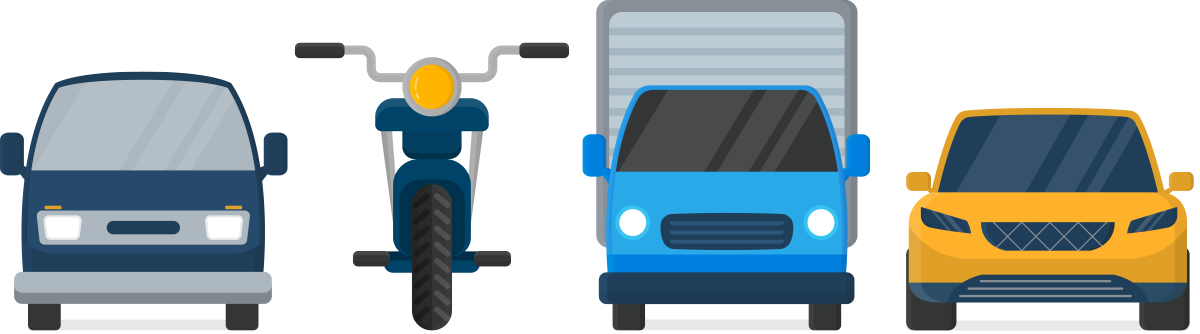
\includegraphics[width=0.5\textwidth]{Images/chapter_15/section_4954864321036288/5727805716561920.png}
\end{minipage}

% \vspace{-1.0\baselineskip}
\noindent
\begin{minipage}[t]{0.48\textwidth}\vspace{0pt}
\begin{itemize}
\item
\textbf{R3:} Each vehicle type may have multiple subtypes, such as:

\begin{itemize}
\item
\textbf{Cars}: Economy, Luxury, Standard, Compact, Intermediate, Full size, Premium
\item
\textbf{Vans}: Passenger, Cargo
\item
\textbf{Motorcycles}: Standard, Cruiser, Touring, Sports, Off-road, Dual purpose
\item
\textbf{Trucks}: Light-duty, Medium-duty, Heavy-duty
\end{itemize}
\item
\textbf{R4:} The system must record every reservation, including the customer details and the date/time a vehicle is issued.
\item
\textbf{R5:} The system can track and report the number of vehicles each customer has rented, including rental history and active reservations.
\item
\textbf{R6:} Customers can cancel their reservations at any time before the pickup date, subject to company policies.
\item
\textbf{R7:} The system maintains a vehicle log to track all significant events related to each vehicle (e.g., maintenance, repairs, accidents, assignments, or status changes).
\end{itemize}
\end{minipage}
\hfill
\begin{minipage}[t]{0.48\textwidth}\vspace{0pt}
\centering
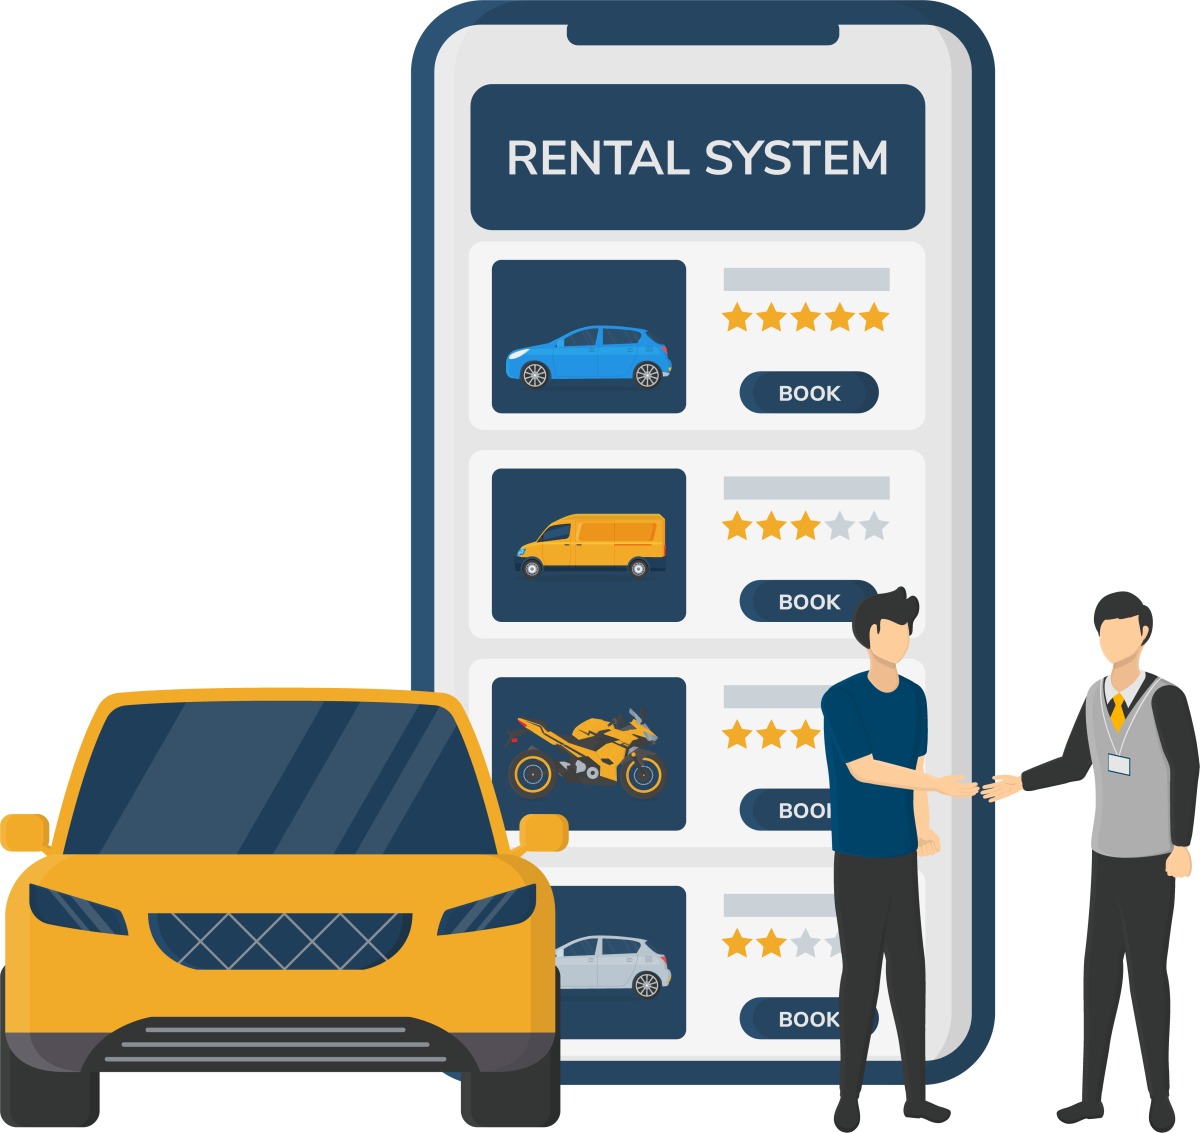
\includegraphics[width=0.5\textwidth]{Images/chapter_15/section_4954864321036288/5546693069373440.png}
\end{minipage}

% \vspace{-1.0\baselineskip}
\noindent
\begin{minipage}[t]{0.48\textwidth}\vspace{0pt}
\begin{itemize}
\item
\textbf{R8:} Customers can add equipment to their reservations, such as a ski rack, child seat, or navigation system.
\item
\textbf{R9:} Customers can add extra services to their reservations, including a driver, Wi-Fi, or roadside assistance.
\end{itemize}
\end{minipage}
\hfill
\begin{minipage}[t]{0.48\textwidth}\vspace{0pt}
\centering
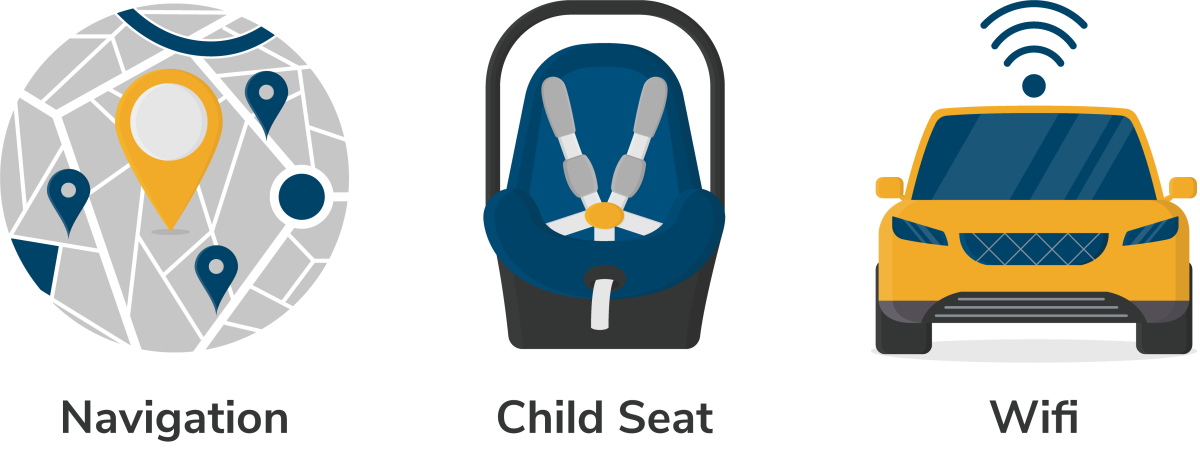
\includegraphics[width=0.5\textwidth]{Images/chapter_15/section_4954864321036288/5981447694581760.png}
\end{minipage}

% \vspace{-1.0\baselineskip}
\noindent
\begin{minipage}[t]{0.48\textwidth}\vspace{0pt}
\begin{itemize}
\item
\textbf{R10:} If a vehicle is not returned by the due date, the system must notify the customer and automatically generate a fine according to company policy.
\item
\textbf{R11:} Users can search for vehicles by type, model, features, or availability at specific locations and dates.
\item
\textbf{R12:} The system must support the management of multiple branches in different cities and locations
\item
\textbf{R13:} Each branch must maintain a record of parking stalls for vehicles at that location, including current status (occupied, available, reserved).
\item
\textbf{R14:} The system should securely process payments, refunds, and fines using multiple payment methods (cash, card, online).
\item
\textbf{R15:} The customer shall be able to make payment for the car rental in both scenarios: when making the reservation and when returning the vehicle. The system should validate both.
\end{itemize}
\end{minipage}
\hfill
\begin{minipage}[t]{0.48\textwidth}\vspace{0pt}
\centering
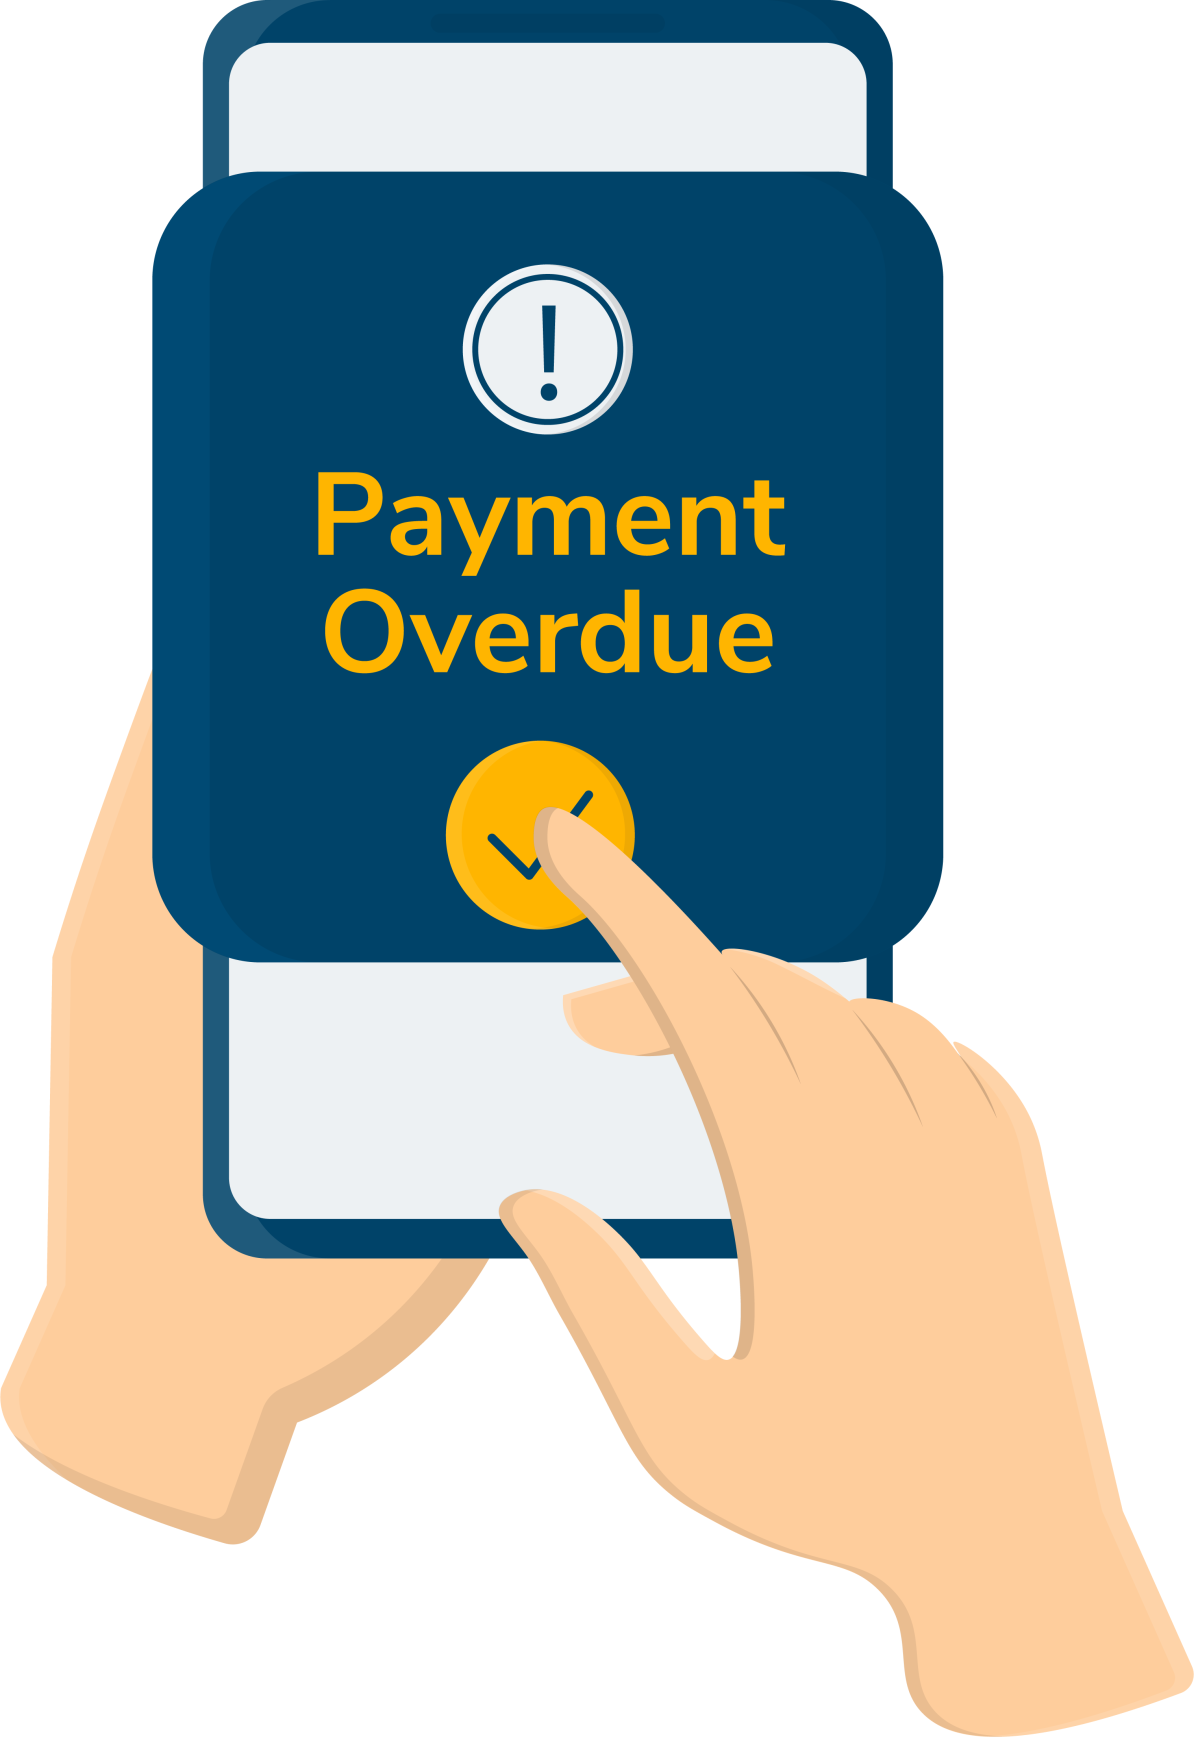
\includegraphics[width=0.5\textwidth]{Images/chapter_15/section_4954864321036288/5035107163570176.png}
\end{minipage}

We've identified our requirements for the problem. In the next lesson, we'll define different use cases of our car rental system.

% End of section content